\documentclass[compress]{beamer}

\usepackage{lmodern}
\usepackage{hyperref}
\usepackage{graphicx}
\usepackage{minted}
\usepackage{epstopdf}
\usepackage{ulem}

\title{Git gud}
\subtitle{Git voor beginners}
\author{Sticky: CommIT}
\date{31 oktober 2016}

\usetheme{Frankfurt}
\usecolortheme{dove}

\setbeamertemplate{section in toc}{\inserttocsectionnumber.~\inserttocsection}
\setbeamertemplate{itemize items}[default]
\setbeamertemplate{enumerate items}[default]

% ToC invoegen aan het begin van elke sectie.
\AtBeginSection
{
  \begin{frame}
      \tableofcontents[currentsection,hideallsubsections,subsubsectionstyle=hide]
    \end{frame}
}
% Bron: https://en.wikibooks.org/wiki/LaTeX/Presentations

\definecolor{light-gray}{gray}{0.90}

\begin{document}

\frame{\titlepage}
\frame{
	\frametitle{Slides zelf erbij houden?}
	\url{http://j.mp/gitgudpdf}
}

\section{Waarom \& hoe git?}

\subsection{Version control}
\begin{frame}{Wat is version control?}
	Op een niet-onhandige manier:
		\begin{itemize}
			\item Code delen met meerdere mensen
			\item Geschiedenis bijhouden / terugdraaien
			\item Veranderingen (evt. over langere tijd) zichtbaar maken
			\item Overzicht van wie wat veranderde
		\end{itemize}
\end{frame}

\subsection{Waarom git?}
\begin{frame}{Waarom git?}
	\begin{itemize}
		\item Distributed:
			\begin{itemize}
				\item Je hebt zelf (standaard) de gehele geschiedenis
				\item Je kan zonder internet werken
			\end{itemize}
		\item Integrity: bestanden kunnen niet veranderen zonder dat git het merkt
		\item Moeilijk om data te vernietigen (`kwijt' kan maar dan moet je beter opletten)
		\item Non-lineair: kan veel dingen naast elkaar starten (en weer weggooien)
		\item Veel diensten op gebouwd: Github, Travis, \ldots
	\end{itemize}
\end{frame}

\begin{frame}{Waarom command line?}
	\begin{itemize}
		\item Hetzelfde over alle platforms
		\item GUIs gebruiken zelfde namen voor dingen
		\item (Er zijn 2 meegeleverde GUI-opties)
	\end{itemize}
	Goede GUIs: zie \href{https://git-scm.com/downloads/guis}{de site van git}
\end{frame}

\section[Structuur]{Structuur van Git}
\subsection{Locaties}
\begin{frame}
	3 plekken waar je gegevens zitten:\\
	\vspace{.5cm}
	\begin{tabular}{ll}
		 Working directory			& pas je aan, normale map\\
		 Staging area				& bestanden die je gaat committen\\
		 Repository / \texttt{.git/}&Bevat metadata, objecten
	\end{tabular}
	% edit-stage-commit cyclus
\end{frame}

\subsection{Gegevensstructuur}
\begin{frame}{Wat slaat git op?}
	Geen lijst van wijzigingen, maar kopie\"en (snapshots):
	\begin{center}
		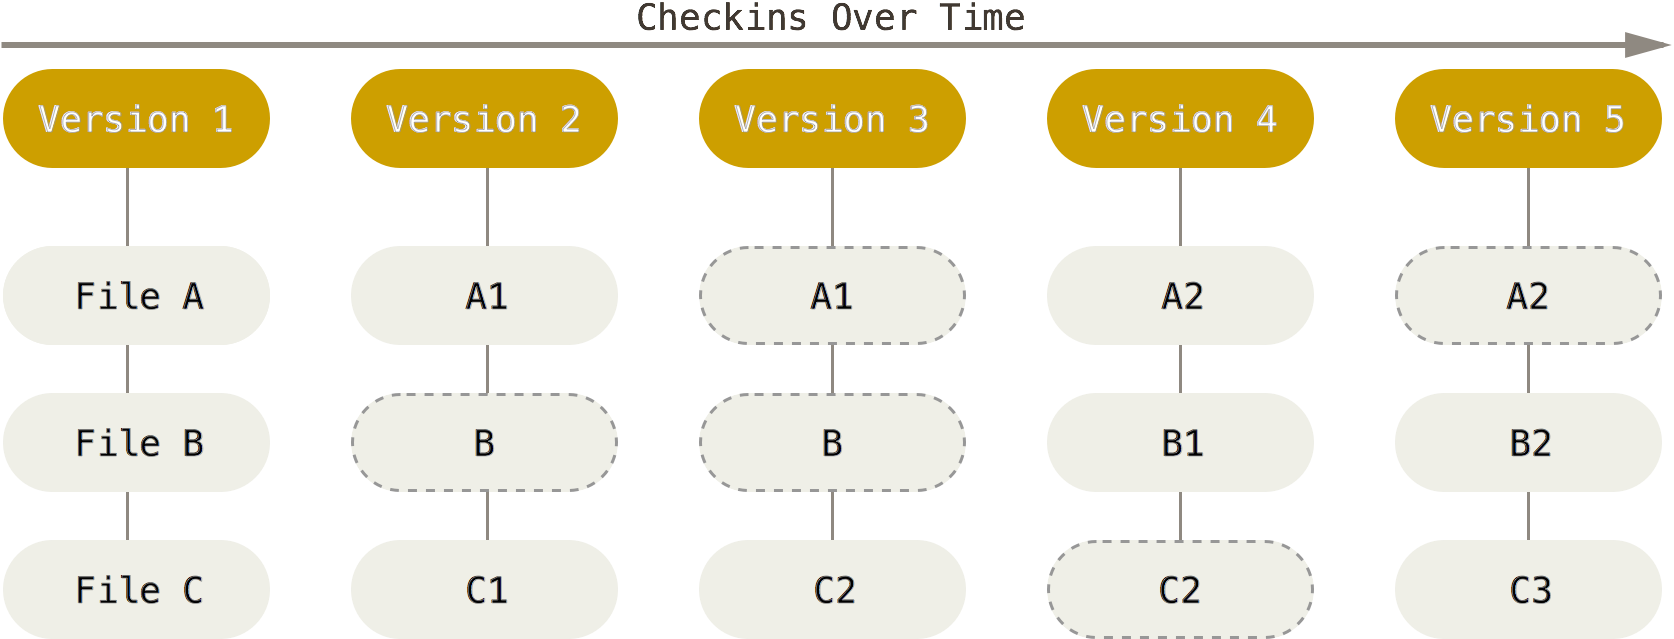
\includegraphics[width=\textwidth]{images/snapshots.png}
	\end{center}
	%(Een version komt hier overeen met een commit, die dus wijst naar versch. versies van bestanden)
\end{frame}

\begin{frame}{Commit}
	\begin{itemize}
		\item Info over jou: (gebruikers)naam + email
		\item Bericht: (hopelijk) korte samenvatting van wat er veranderde
		\item Verwijzing naar set snapshots van bestanden (objects)
		\item Voorganger (merge: 2, initial: 0)
		\item Unieke id (40 tekens)
	\end{itemize}
	\alert{Later (wanneer gedeeld met externe server) niet meer aan (te) passen!}
\end{frame}

\section[Get git]{Installatie}

\subsection{Download}
\begin{frame}
	\begin{itemize}
		\item Windows: \url{https://git-scm.com/download/win}
			\begin{itemize}
				\item \small{Maak snelkoppeling naar git-bash in \tt{Program Files/Git/cmd}}
			\end{itemize}
		\item Mac: \url{https://git-scm.com/download/mac}
		\item Linux: gebruik je package manager
	\end{itemize}
\end{frame}

\subsection{Configureren}
\begin{frame}{Instellen (doemoment!)}
	Installeer Git van de site \url{https://git-scm.com}\\

	Open Git Bash en voer in wie je bent:
	\begin{itemize}
		\item \tt{git config --global user.name "Lars Verhoeven"}
		\item \tt{git config --global user.email "user@example.com"}
	\end{itemize}
	{\small\alert{Wordt aan iedere commit verbonden die je maakt!}}\\

	\texttt{git config --global color.ui auto}\\
	\texttt{git config --global core.editor nano}\\

	Als je minder vaak om je wachtwoord wil worden gevraagd (bij externe servers):

	\begin{itemize}
		\item \tt{git config --global credential.helper cache}
		\item \tt{git config --global credential.helper "cache --timeout=3600"}
	\end{itemize}
\end{frame}

\section{Basisacties}

\subsection{Repository aanmaken}
\begin{frame}[fragile]{Repository maken}
	\begin{enumerate}
		\item Open terminal (windows: \alert{git-bash})
		\item \texttt{cd} naar map die je wil bijhouden
			(of \texttt{mkdir} een nieuwe)
		\item \texttt{git init}
		\item \texttt{git status}
	\end{enumerate}
	Als het goed is zie je nu \alert{niet}:
	\begin{minted}[bgcolor=light-gray]{text}
fatal: Not a git repository or 
	any of the parent directories: .git
	\end{minted}
\end{frame}

\subsection{Bestanden laten bijhouden}
\begin{frame}[fragile]{Je eerste commit}
	\begin{enumerate}
		\item \texttt{git status}: overzicht van wat afwijkt van opgeslagen
		\item Bekijk 'untracked files'
		\item \texttt{git add bestand1 bestand2 map1}\\ of:
			\texttt{git add .}\\
			(opgeven van map pakt alles erin, . is huidige map)
		\item \texttt{git commit}, voer bericht in, opslaan en sluiten\\
			(of: \texttt{git commit -m "Eerste commit"})
	\end{enumerate}
	Resultaat: 
	\begin{minted}[bgcolor=light-gray]{text}
[master 1234abc] Eerste commit
x files added
	\end{minted}
\end{frame}

\begin{frame}{Bestanden ontstagen}
	\texttt{git add} is ongedaan te maken:\\
	\texttt{git reset HEAD <bestand>}\\
	(Zie ook de tekst van \texttt{git status})
\end{frame}

\begin{frame}{Help mijn commit is niet goed}
	\texttt{git commit --amend}:
	\begin{itemize}
		\item Commit message nog aanpassen
		\item Files die niet gestaged waren
	\end{itemize}
	\alert{Commit moet nieuwste en niet gedeeld zijn}
\end{frame}

\subsubsection{Wat is hier gebeurd?}
\begin{frame}{Wat is er nu eigenlijk gebeurd?}
	\begin{center}
		\includegraphics[width=.7\textwidth]{graphs/basis1.eps}<1>
		\includegraphics[width=.7\textwidth]{graphs/basis2.eps}<2>
	\end{center}
\end{frame}

\subsubsection{Commit messages}
\begin{frame}{Commit message}
	Iedere commit heeft een message:
	\begin{itemize}
		\item Subject line
		\item Lege regel
		\item Body
	\end{itemize}
\end{frame}

\begin{frame}{Commit message schrijven}
	Niet verplicht, wel handig/netjes:
	\begin{enumerate}
		\item Scheid subject en body met een lege regel (!)
		\item Subject niet langer dan 50 tekens
		\item Subject beginnen met een hoofdletter
		\item Subject niet eindigen met een punt
		\item Subject imperatief: `Verwijder alles' i.p.v. `Verwijdert alles'
		\item Regels van de body op 72 tekens lang
		\item Zet \emph{wat} en \emph{waarom} in de body, \emph{hoe} gebeurt automatisch
	\end{enumerate}
	% Bron: http://chris.beams.io/posts/git-commit/
\end{frame}

\begin{frame}
	\begin{center}
		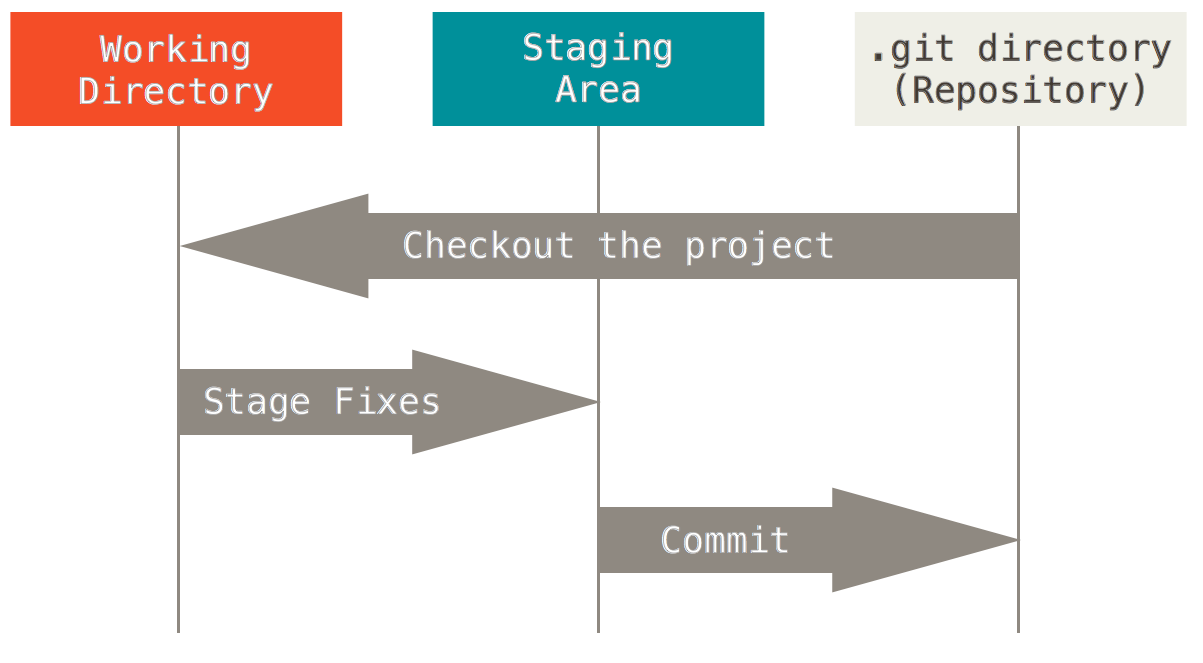
\includegraphics[width=\textwidth]{images/areas}
	\end{center}
	\begin{itemize}
		\item \texttt{git add} $\rightarrow$ 'Stage Fixes'
		\item \texttt{git commit} $\rightarrow$ 'Commit'
	\end{itemize}
\end{frame}

\subsubsection{Bestanden negeren}
\begin{frame}[fragile]{Bestanden negeren}
	\begin{itemize}
		\item \texttt{git status} geeft onbekende bestanden altijd aan
		\item Oplossing 1: \texttt{.gitignore}:
	\end{itemize}
	\begin{minted}[bgcolor=light-gray]{text}
# alle bestanden in de map bin
bin/*

# alle .exe
*.exe

# maar wel dinges.exe
!dinges.exe
	\end{minted}

	(\texttt{.gitignore} moet wel gecommit worden)
\end{frame}

\begin{frame}{Bestanden alleen voor jezelf negeren}
	\texttt{.git/info/exclude}:
	\begin{itemize}
		\item Alleen op je eigen kopie van repo
		\item Zelfde syntax als \texttt{.gitignore}
	\end{itemize}
\end{frame}

\subsection{Geschiedenis bekijken}
% git log
\begin{frame}{log}
	\begin{tabular}{ll}
		\texttt{git log}& Bekijk geschiedenis van commits (\texttt{--reverse})\\
		\texttt{git show}& Bekijk veranderingen in commit, standaard nieuwste
	\end{tabular}
\end{frame}

% git diff
\begin{frame}{git diff}
	\begin{tabular}{ll}
		\texttt{git diff}&Toon veranderingen in tracked files (unstaged)\\
		\texttt{git diff --staged}&Toon veranderingen klaargezet voor commit\\
		\texttt{git diff HEAD\^}&Toon veranderingen sinds vorige commit
	\end{tabular}
\end{frame}

% git show
\begin{frame}{git show}
	\begin{tabular}{l l}
		\texttt{git show}&Toon info over vorige commit\\
		\texttt{git show id}&Toon info over commit \texttt{id}\\
	\end{tabular}
\end{frame}

\subsection{Overzicht}
\begin{frame}{Overzicht}
	{ \footnotesize
	\begin{tabular}{ll}
		\texttt{git init}					& maak een nieuwe repository \\
		\texttt{git status} 				& bekijk wat git denkt dat er aan de hand is \\
		\texttt{git add file map \ldots}	& bestanden klaarzetten voor commit (stagen)	\\
		\texttt{git commit} 				& klaargezette bestanden in geschiedenis zetten (committen)\\
		\texttt{git reset file}		    	& bestanden ontstagen (omgekeerde van \texttt{add})	\\
		\hline
		\texttt{git diff}					& Veranderingen in tracked files					\\
		\texttt{git diff --staged}			& Wat ga ik committen? (wat is staged?)				\\
		\texttt{git diff HEAD\^}			& Wat is er veranderd sinds de vorige commit?		\\
		\hline
		\texttt{git log}					& Bekijk vorige commits								\\
		\texttt{git show id}				& Bekijk commit \texttt{id} in detail
	\end{tabular}
	}
	Doen:
	\begin{enumerate}
		\item Maak een lege map met repo
		\item Download \url{https://j.mp/gitgud-ex1}
		\item Add en commit
		\item Bug: 16 moet \texttt{`date +\%d`} zijn, repareer en commit
		\item \texttt{bash simpelscript.sh}
	\end{enumerate}
\end{frame}

\section[Ongedaan]{Dingen ongedaan maken}

\subsection{Bestand terugdraaien naar onbewerkt}
\begin{frame}{Bestand terug naar vorige commit}
	\texttt{git checkout -- <bestand>} \\
	\alert{Omdat dit niet gecommit was ben je je wijzigingen kwijt!}
\end{frame}

\subsection{Bestanden terugdraaien naar eerdere versie}
\begin{frame}{Bestand(en) terug naar eerdere versie}
	\begin{itemize}
		\item \texttt{git checkout <hash> <bestand>}: enkele bestanden, staget
		\item \texttt{git checkout HEAD <bestand>}: vorige ongedaan maken
		\item \texttt{git checkout <hash>}: detached HEAD
		\item \texttt{git checkout master}: detached HEAD ongedaan maken
	\end{itemize}
	%(Hash opzoeken met git log, of: \texttt{HEAD\^, HEAD\^\^, HEAD\textasciitilde 5})
\end{frame}

\begin{frame}{Detached HEAD in plaatjes}
	\begin{center}
		\includegraphics[width=.7\textwidth]{graphs/basis3.eps}<1,3>
		\includegraphics[width=.7\textwidth]{graphs/basis4.eps}<2>
	\end{center}
	\only<1>{Basisstaat van eerder}
	\only<2>{\texttt{git checkout B}}
	\only<3>{\texttt{git checkout master} (niet \texttt{C}!)}
\end{frame}

\subsection{Commits ongedaan maken}
\begin{frame}{git revert}
	\begin{itemize}
		\item \texttt{git revert <hash>}: maak nieuwe omgekeerde commit
		\item Safe: reverts van reverts van reverts kan je reverten
	\end{itemize}
\end{frame}

\begin{frame}{git reset}
	Veilig:
	\begin{itemize}
		\item \texttt{git reset}: unstage alles
		\item \texttt{git reset <bestand>}: unstage bestand
	\end{itemize}
	\alert{Onveilig:}
	\begin{itemize}
		\item \texttt{git reset --hard}: \texttt{checkout --} op hele working directory
		%\item \texttt{git reset <commit>}: verwijder alle commits na \texttt{<commit>}, laat WD staan
		%\item \texttt{git reset --hard <commit>}: \alert{dat is pech, data weg!}
	\end{itemize}
	%\alert{Reset alleen lokale dingen!}
\end{frame}

\begin{frame}{git clean}
	\alert{Verwijdert untracked bestanden!}
	\begin{itemize}
		\item \texttt{git clean -n}: dry run
		\item \texttt{git clean -x}: inclusief genegeerd
		\item \texttt{git clean -d}: untracked mappen
		\item \texttt{git clean --force}: \alert{poef}
	\end{itemize}
	(Soms beter om een snapshot van je branch te downloaden)
\end{frame}

\subsection{Overzicht}
\begin{frame}{Overzicht}
	{ \footnotesize
	\begin{tabular}{ll}
		\texttt{git checkout -- bestand}		& bestand terug naar vorige commit	\\
		\texttt{git commit} & klaargezette bestanden in geschiedenis zetten (committen)\\
		\texttt{git reset}	& bestanden ontstagen (omgekeerde van \texttt{add}
	\end{tabular}
	}
	Doen:
	\begin{enumerate}
		\item Ga terug naar je repo van eerder
		\item Run het script (\texttt{bash simpelscript.sh}) $\rightarrow$ untracked file
		\item \texttt{git clean -n}, \texttt{git clean -f}
		\item \texttt{.gitignore} maken met \texttt{laatstekeer.txt}
		\item \texttt{git clean -n} : bestand weg?
		\item \texttt{git clean -xn}, \texttt{git clean -xf}
		\item Commit je \texttt{.gitignore}
	\end{enumerate}
	Cheat sheet van eerdere dingen? \url{http://overapi.com/git}
\end{frame}

\section{Verschillende versies naast elkaar}[Branches]

\frame{
	\texttt{git status}: On branch master \ldots
}

\section{Samenwerken}

\subsection{Remotes}
\begin{frame}{Remotes}
	Remote: andere (volledige) git repo met gedeeld punt in geschiedenis
	\begin{itemize}
		\item \texttt{git remote -v}: toon remotes met url
		\item \texttt{git remote add <naam> <url>}: \texttt{naam} wordt alias voor \texttt{url}
	\end{itemize}
	Goede plekken om je repository te hosten:
	\begin{itemize}
		\item Github: veel gebruikt, Travis, gratis student account (private repo's beperkt)
		\item Bitbucket: alternatief voor Github, onbeperkt private repo's
		\item UU GitLab: intern voor de UU, mailinglijst, onbeperkt private repo's
	\end{itemize}
\end{frame}

\subsection{SSH keys}
\begin{frame}{SSH keys}
	\begin{enumerate}
		\item Open terminal/Terminal/git-bash
		\item \texttt{ssh-keygen}
		\item Edit je \texttt{.bashrc} of \texttt{.profile}\\
			Voeg toe: \texttt{eval `ssh-agent`}
	\end{enumerate}
\end{frame}

\subsection{Bestaande repo overnemen}
\begin{frame}{git clone}
	Kopieer repository en maak remote `origin'
	\begin{itemize}
		\item \texttt{git clone <url>}
		\item \texttt{git clone <url> <map>}
	\end{itemize}
	Als niet je eigen repo en wel toevoegingen maken: forken
\end{frame}

\subsection{Wijzigingen binnenhalen}
\begin{frame}{git fetch}
	Kopieer commits van een remote naar je repo
\end{frame}

\section[Tips]{Tips en tricks}

\begin{frame}{git alias}
	Maak verkortingen voor commando's:
	\begin{itemize}
		\item \texttt{git config alias.overzicht "log --all --graph --decorate --oneline"}
		\item \texttt{git config alias.unstage "reset HEAD"}
	\end{itemize}
	Maak aliases global (voor al je git repo's op die computer) met \texttt{git config --global \ldots}
\end{frame}

\begin{frame}{git grep}
	Zoeken in alle tracked files:
	\begin{itemize}
		\item \texttt{git grep "Zoeken"}
		\item \texttt{git grep -i "zOEkEn"} hoofdletterongevoelig
		\item \texttt{git grep -n "Zoeken"} regelnummer
		\item \texttt{git config --global alias.zoek "grep -ni"} alias voor beide
	\end{itemize}
\end{frame}

\begin{frame}{git help}
	Uitgebreide handleiding: \texttt{git help [commando]}
\end{frame}

\begin{frame}{Voorbij deze workshop}
	\begin{itemize}
		\item \url{https://git-scm.com/book} Pro Git
		\item \url{https://codecademy.com/learn/learn-git}
		\item \url{https://www.atlassian.com/git/tutorials/}
		\item \url{https://overapi.com/git/} Cheat sheet!
	\end{itemize}
\end{frame}

\begin{frame}{Dat was het dan}
	`Ga heen en git gud!'
\end{frame}


\end{document}
